\chapter{Recording History} \label{sec:history}

Up until this point, the presented work has focused on experimentation, research, and prototyping. Chapters \ref{sec:heatpumpcollection} through \ref{sec:simulationprototype} identified key use cases, requirements, and architectures for processing live data. 
\Cref{sec:heatpumpcollection} identified that while data collection is straightforward, there are limitations to the data that can be collected. Often, custom logic for inference or sensor fusion will be required. \Cref{sec:architectureresearch} concluded that IDAES is capable of supporting dynamic modelling, surrogate modelling, optimisation, and control, but that these features mean different things in the context of live data processing compared to offline simulation. 
\Cref{sec:simulationprototype} demonstrated that the Ahuora Simulation Platform could be integrated with a real-time data processing system for steady-state modelling with relatively little effort, as long as there is a standardised API, and provided techniques to do so. However, much more complexity arises when combining all these concepts together, and when balancing the needs of the engineer's workflow with the operator's workflow.

This chapter focuses on iteratively developing the Ahuora Simulation Platform to support live data processing, and testing these developments on the Heat Pump Dryer Model. 

\section{Purpose}

To better understand the tradeoffs of a more integrated platform, it was decided to implement a solve history system. This would allow the user to view the results of previous simulations, and compare them. It is a useful feature for the Ahuora Simulation platform as a standalone tool, but it can also be used to record the results of the real-time data processing system. A simple dashboard is created to view past solving results, which can show how the system has changed over time. Significant advantages revealed by this approach demonstrate the potential for development of a more integrated system. Beyond such a development, this approach also provides insight into how to break the system apart while retaining similar functionality.


\section{Development} \label{sec:recordinghistorydevelopment}

The Ahuora Simulation platform stores all simulation results in a database after they are returned from IDAES. Initially, only one entry was maintained with data overwritten by each subsequent flowsheet solve. To enable storing history of previous solves, a table was created to store the results of each previous solve, and new entries were automatically added each time the simulation was run. Then, a user interface was created to view the results of the simulations.

% TODO:include some screenshots of the data tables, and the chart creation system.

\begin{figure}
    \centering
    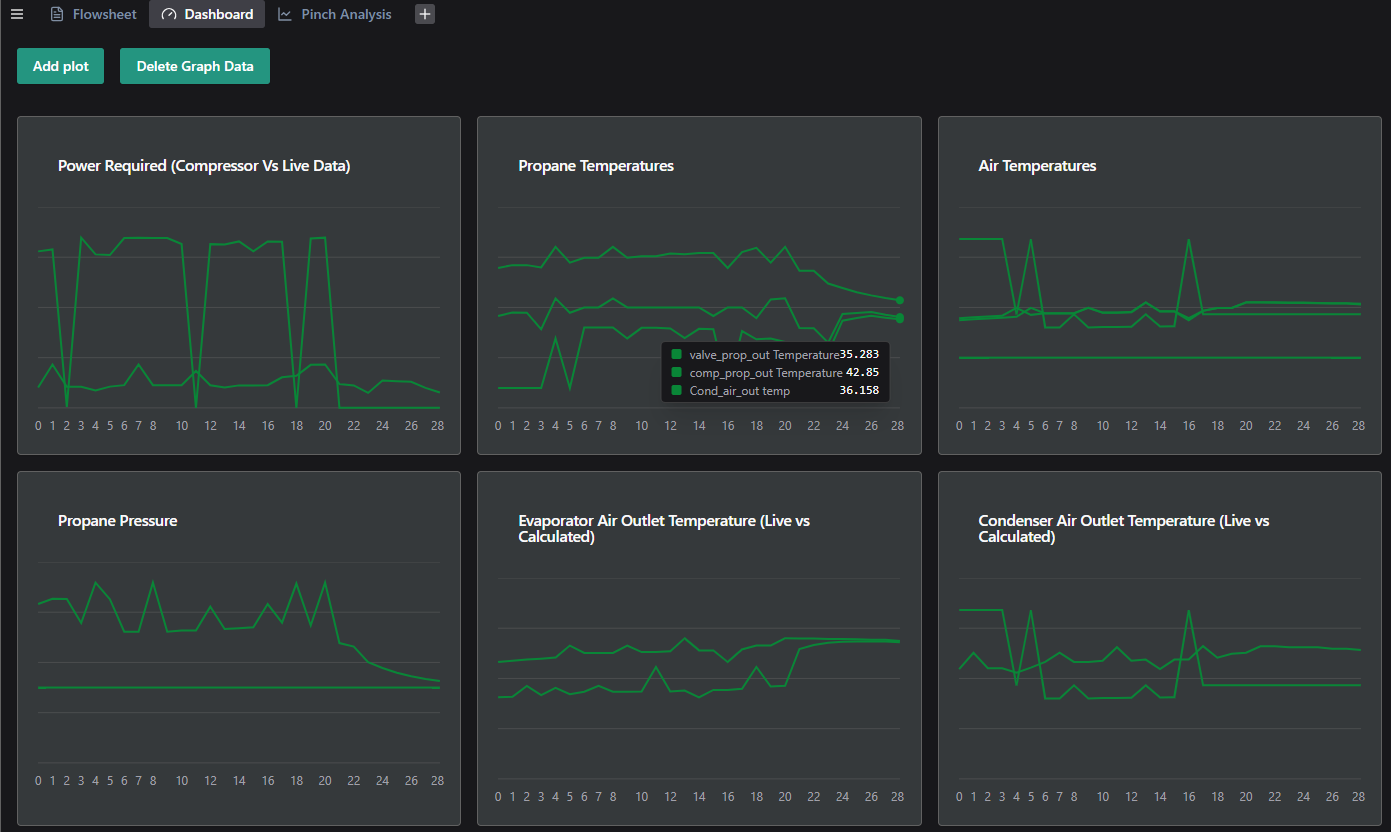
\includegraphics[width=\textwidth]{livedatadashboard.png}
    \caption{Live Data Dashboard in the Ahuora Digital Twin Platform}
    \label{fig:livedatadashboard}
\end{figure}

A seperate tab has been added to the Ahuora Simulation Platform to show the graphs of previous simulation results. This is illustrated by \Cref{fig:livedatadashboard}, which shows the user interface that was created as part of the development, with a number of manually created graphs for the heat pump dryer. 


\section{Testing}

The data collection scripts from \Cref{sec:heatpumpcollection} were updated to store the results in the Ahuora Simulation Platform instead of InfluxDB, using methods previously outlined in \Cref{sec:simulationprototype}. A heat pump was modelled in the Ahuora Simulation Platform. At this stage, the Ahuora Simulation Platform was able to reliably solve heat pumps with pure chemical components, and as the heat pump dryer used propane as a refrigerant, it was a good test case. 


\begin{figure}
    \centering
    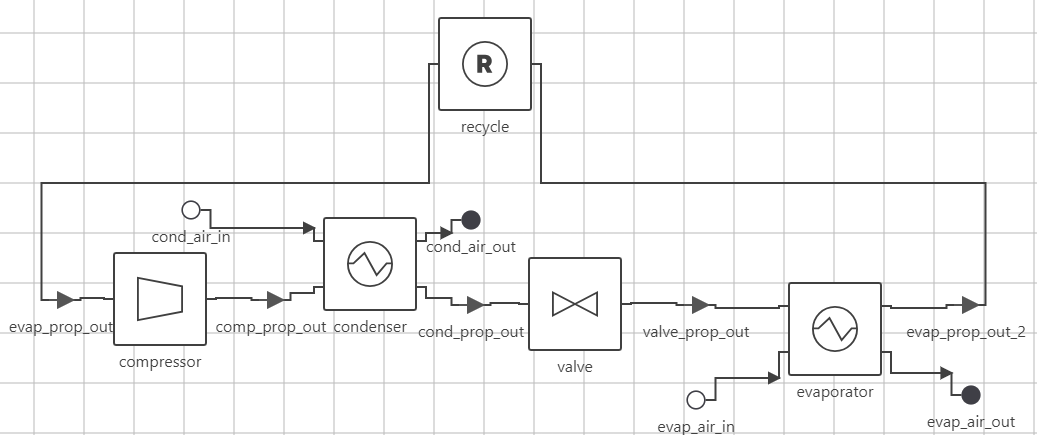
\includegraphics[width=\textwidth]{heatpumpmodel.png}
    \caption{Heat Pump Model used for live data}
    \label{fig:heatpumpmodel}
\end{figure}

\Cref{fig:heatpumpmodel} shows the heat pump model built in the Ahuora Simulation platform for this test. There are four unit operations in this model:

\begin{itemize}
    \item The compressor pressurizes the propane gas, heating it up at the same time. 
    \item The condenser cools down the propane, and the propane liquifies. The heat that leaves the propane moves into the internal drum of the dryer.
    \item The propane then moves through the valve, which reduces the pressure significantly. This causes the propane to vaporise, and the temperature further decreases to well below room temperature.
    \item Lastly, the propane moves through the evaporator, where it collects heat from the ambient surroundings, back to its original temperature.
    \item The recycle block is not a unit operation, but it specifies that the propane from the evaporator is fed back round into the inlet of the compressor. This means that the temperature, pressure, and flow rate out of the evaporator is the same as into the compressor.
\end{itemize}

The complexity arose in linking the data from the real-world sensors to the data from the simulation. In the data collection configuration the dryer was set up for, a sensor is used to read the temperature of the propane leaving the compressor, and out of the evaporator. Additionally, air temperatures are also measured, and the total power of the dryer is measured. Other properties required to calculate the flowsheet needed to be hardcoded, as shown in \Cref{tab:tempconditions}. 
The sensor readings that were measured, but not used in calculating the flowsheet are shown in \Cref{tab:liveprops}. The reason not all sensor data was used is twofold: first, the air temperature readings would also require knowing the flow rate of the air and propane, which were unknown. Second, they would over-define the simulation which would make solving infeasible. 
As there were no pressure sensors, the pressure of the propane could not be measured. Thus, hand-calculations were performed to calculate what feasible pressures the propane would be at for it to boil below room temperature and at approximately 70~\degree~C. The model performance did not always exactly reflect real-world conditions, but it was accurate enough for proof of concept purposes.

The Ahuora Simulation Platform did not initially support specifying the outlet temperature of a compressor or valve, when these make more sensible calculation modes than outlet pressure for our avaliable live data. These were added to support this workflow.

\begin{table}[htbp]
    \centering
    \caption{Specified properties in heat pump model}
    \label{tab:tempconditions}
    \begin{tabular}{|c|c|c|}
        \hline
            \textbf{Unit Operation} & \textbf{Property} & \textbf{Source} \\
            \hline
            Compressor & Outlet Temperature & Probe Temperature Sensor \\
            Compressor & Isentropic Efficiency & Hardcoded to 100\% \\
            Condenser & Air Inlet Temperature & Hardcoded to 20 \degree C \\
            Condenser & Propane Outlet Temperature & Hardcoded to 40 \degree C \\
            Valve & Outlet Pressure & Hardcoded to 6 bar \\
            Evaporator & Air Inlet Temperature & Dryer Temperature Sensor \\
            Evaporator & Propane Outlet Temperature & Probe Temperature Sensor \\
        \hline
    \end{tabular}
\end{table}

\begin{table}[htbp]
    \centering
    \caption{Other sensor readings, not used in solving}
    \label{tab:liveprops}
    \begin{tabular}{|c|c|c|}
        \hline
            \textbf{Unit Operation} & \textbf{Property} & \textbf{Reason} \\
            \hline
            Condenser & Air Outlet Temperature & Can be calculated from propane outlet temperature \\
            Evaporator & Air Outlet Temperature & Can be calculated from propane outlet temperature \\
            Entire Dryer & Power Usage & Doesn't map cleanly to one property \\
        \hline
    \end{tabular}
\end{table}

As the Ahuora Simulation Platform can only store solving results, additional ``dummy'' unit operations were added to the flowsheet to store the other sensor readings mentioned in \Cref{tab:liveprops}.

The live data processing script was then started and run with the developed model as specified.
While the model was thermodynamically valid as it was built, and could solve correctly, the integration of live data quickly resulted in the model failing to solve.
Sometimes, IDAES would fail to initialize the models. Other times, the IPOPT solver found that either the model was infeasible, or the problem failed in restoration phase (which could be from poor scaling, inaccurate results, or it could not find a feasible starting point for solving).


There are several potential causes for such failures. One possibility is hardcoded data. A likely source of failure is the discrepancies between the dynamic nature of the physical heat pump dryer and the steady state nature of the model. It takes time for the dryer to reach steady state, as it initially starts at room temperature. The model is trying to solve everything as a steady state - wheras in reality it takes time for changes in temperature to propagate through the entire system. 

Additionally, the dryer has it's own built-in control system, and it is not always running. When the dryer is not running, the simulation model is not correct. This may result in infeasible solutions. 



\section{Results \& Insights}

This identified a number of problems with the current ways of handling live data.

Firstly, there needs to be a better way to handle failed solves. The only data that the flowsheet history stored was data on successful solves. When debugging solving, it would be much more useful to store successful and failed solve states. However, it may not make sense to store failed solve results in the Ahuora Simulation Platform, as the results from idaes are useless in that case. 
A potential solution can be found in the form of an external data pipeline to manage this.
Additionally, the Ahuora Simulation Platform only stores properties of unit operations in the solve, making it hard to add additional data such as timestamps, or other data collected from sensors. It doesn't provide a fully-fleged data processing platform. 
In the test example, additional "dummy unit operations" disconnected from the main flowsheet were used to store the data, but this is a workaround and should not be viewed as a long term solution.
It also would not be appropriate for other types of data, e.g if images were taken of the plant over time. From this, we can conclude that it is not appropriate for the Ahuora Digital Twin platform to form the entire knowledge base of a plant.

Secondly, the methods of specifying unit operations can vary, and the Ahuora Simulation Platform will need to support a wide number of calculation modes - in this case, an additional calculation mode (Outlet Temperature) had to be added to the compressor in order to solve the model. On discussing these results with other colleagues who are chemical engineers, they mentioned that it is common to have to calculate properties in roundabout ways. 
For example, you can calculate temperature by how much a pipe expands, or the pressure of a valve outlet from its temperature, assuming it's in the two-phase region (transitioning between liquid and gas) and is a pure fluid. The Ahuora Simulation Platform has ``Specification Blocks'' on it's roadmap of future development, which allow specifying arbitrary relationships between variables. This may help with such scenarios. Additionally, it may be worth introducing a preprocessing step into the workflow prior to feeding the calculated values into the Ahuora Simulation Platform.

There was a lot of data that could not be used in the Ahuora Simulation Platform due to limited flexibility of existing model specifications. With greater flexibility, the inlet and outlet air temperatures could have been used to calculate the heat capacity of the air streams, or efficiency of the heat exchangers.
Alternatively, overspecified data could be used for sensor fusion as explained in the Literature Review (Appendix \ref{sec:litreview}), using Bayesian statistics to calculate what the most probable true values are and the uncertainty associated with them. 
However, this would significantly increase the complexity of the model; an alternative is to just compare the simulation output to the live data, and flag any significant variations as a problem in a concept drift approach. 
Sensor fusion would likely require bayesian methods to be implemented into the Ahuora Simulation Platforms, comparing variances could be done as a postprocessing step in a seperate software.

%TODO: Link all the use cases together in the proposed system architecture section.
This all provides cause for reflection on the use cases identified in \Cref{sec:researchconclusions}, \Cref{tab:requirements}. 
While both the engineer's use case and the operator's use cases are still valid, there was an assumption that the person setting up the digital twin would be able to easily port an engineer's model (e.g, from the design of a plant) into a digital twin that processes live data; that it would be just a matter of linking the model up with a live data source. 
From this test, it is clear that finding the correct parameters to define a model, and finding a way to link sensor readings up with simulation parameters, is a non-trivial task: it is not as straightforward as a one-to-one mapping. 
Thus, two other use cases should be considered. A ``Data Engineer'' may be a Software Engineer responsible for aggregating data from different sensors (and simulation results) into a single SCADA system or Industrial IoT system. 
A ``Process Engineer'', for want of a better term, may be a Chemical Engineer who is responsible for linking existing simulation models with the IoT data, using their domain specific knowledge to convert the IoT readings from sensor outputs into valid parameters for a simulation model, using sensor fusion or other techniques. 
These need to be considered alongside the requirements of a chemical engineer only focused on design, and an operator only focused on control.

\begin{table}[ht]
    \centering
    \caption{Comparison of a Data Engineer's and a Process Engineer's workflow}
    \begin{tabular}{|c|p{0.35\textwidth}|p{0.4\textwidth}|}
        \hline
        \textbf{Requirement} & \textbf{Data Engineer} & \textbf{Process Engineer} \\
        \hline
        Use Case & Integrating simulation results into company knowledge base & Convert sensor readings into model parameters \\
        \hline
        Skillset & Software, Networking, Data Storage, and Data Processing  & Chemical Modelling, Data Processing \\
        \hline
        Modelling & Doesn't do chemical modelling & Extends the model with sensor fusion \& preprocessing techniques\\
        \hline
        Requirements & Good API to interface with the platform & Easy to use tools and techniques for sensor fusion \\
        \hline
        Historical Data & Needs to store historical data & Needs to test models on historical data \\
        \hline
    \end{tabular}
    \label{tab:morerequirements}
\end{table}


\Cref{tab:morerequirements} summarises the requirements of each of these new use cases. The data engineer is most concerned about integration with existing systems. This would be best serviced by ensuring the data processing platform in Ahuora has simple, clear APIs to ingest data and extract data after solve. The Process Engineer wants easy access to all the sensor data in the factory, and sufficient tooling to be able to convert the sensor data into model parameters. This could be achieved by adding additional model properties to the Ahuora Simulation Platform, but more complex cases may require additional pre/postprocessing outside of the IDAES solver. Exactly what this could entail is highly implementation-specific.

\section{Discussion}

% TODO: Consider how this relates to the previous chapter and how it sets things up to the next chapter, adjust them so they're consistent.

In the previous chapter, \Cref{sec:prototypeinsights} discussed the tradeoffs between doing everything in the Ahuora Platform, and doing as much as possible in an external system. The insights gained in this chapter suggest that the Ahuora Simulation platform alone is insufficient, and that linking with external systems would be required to store results in line with other company data. This also enables more advanced processing techniques to be implemented through custom logic outside of the Ahuora Platform. However, specific techniques that involve extending the mathematical model of the system would be best done in the Ahuora Simulation Platform. A seperate suite of tools to handle a data processing pipeline would best support this, though a full implementation would be a significant undertaking that is beyond the scope of this project. 

Additionally, a Process Engineer, who is not as skilled at software engineering or programming, would be best served by having some data preprocessing tools built into the platform. As an integrated solution, they could test their models on historical data, using platform tools for data processing. A Data Engineer could then be responsible for providing the required live data to the platform, and storing simulation results, without having to deal with the intracacies of the model itself.




\section{Improving Solving Reliability} \label{sec:solvingreliability}

% Talk about why initialisation could be a failing point, how to fix that (e.g remove the recycle, or save initialisation states)
As the solving for the heat pump dryer was not always successful, some additional time was spent to improve the reliability of solving.
This helped to identify relevant preprocessing steps to implement in the platform.
There are a couple of reasons why the solving of the flowsheet was not always successful in the previous section. 

The first reason is that the heat exchangers could be failing to initialise. They are the most complex unit operation, and require appropriate fluid volumes, heat deltas, flow transfer areas, and heat transfer coefficients to be set. If these are not set correctly, the heat exchanger may not initialise. 

As we did not have flow rates for the air inlets in this model, approximate values were being used. Thus including heat exchangers in the model did not provide any more accuracy, and only added complexity. The model was updated with heaters and coolers instead of heat exchangers, which can be solved much more reliably.

The second reason why the model may not have been solving is that the recycle loop was not being initialised correctly. The recycle stream was being set to the same value as the outlet stream, but this creates a continuous loop that the solver may not be able to solve at a steady state as it is classed as a degenerate problem.
In IDAES, tear guesses are used to decompose continuous loops sequentially until the solutions start to converge.
For the next test, the recycle was removed, and the tear guess values were used as the initial conditions. This achieves a similar simulation result, with slightly fewer constraints and much less complexity.

% TODO: picture of the data (look it's not so sparodic anymore) - or of the sequential decomposition routines

When both of these changes were made, the model was able to solve reliably. The results of the simulation were much more consistent, and better reflected the expected behaviour of the heat pump dryer.


While implementing this, another issue was discovered. Because stream properties were being used to store additional live data that was not part of the simulation, sometimes the live data was invalid as a stream condition. This was done so the part of the platform that recorded solve history could be used to display all live data results, not just the simulation results. However, this was not a good solution, as it made the simulation less reliable. This means that either the solve history feature should be updated to handle storing additional metadata, or the live data should be stored in a different way.


% Todo: figure out a bit more of a structure for this

% Maybe mention scaling?

% is there any other preprocessing steps we could do? Should we add specification blocks?

% what does this prove about the architecture?

